\section{Background}

% NOTE: This text is just a short introduction of what is coming in the next 3 subsections, if it is too repetitive we can remove it.

\subsection{SherpaTT}

\begin{figure*}[!htbp]
   \subcaptionbox{
       \label{fig:SensorInputs}Sensor and joint inputs to the Terrain Classifier
       }
       {
           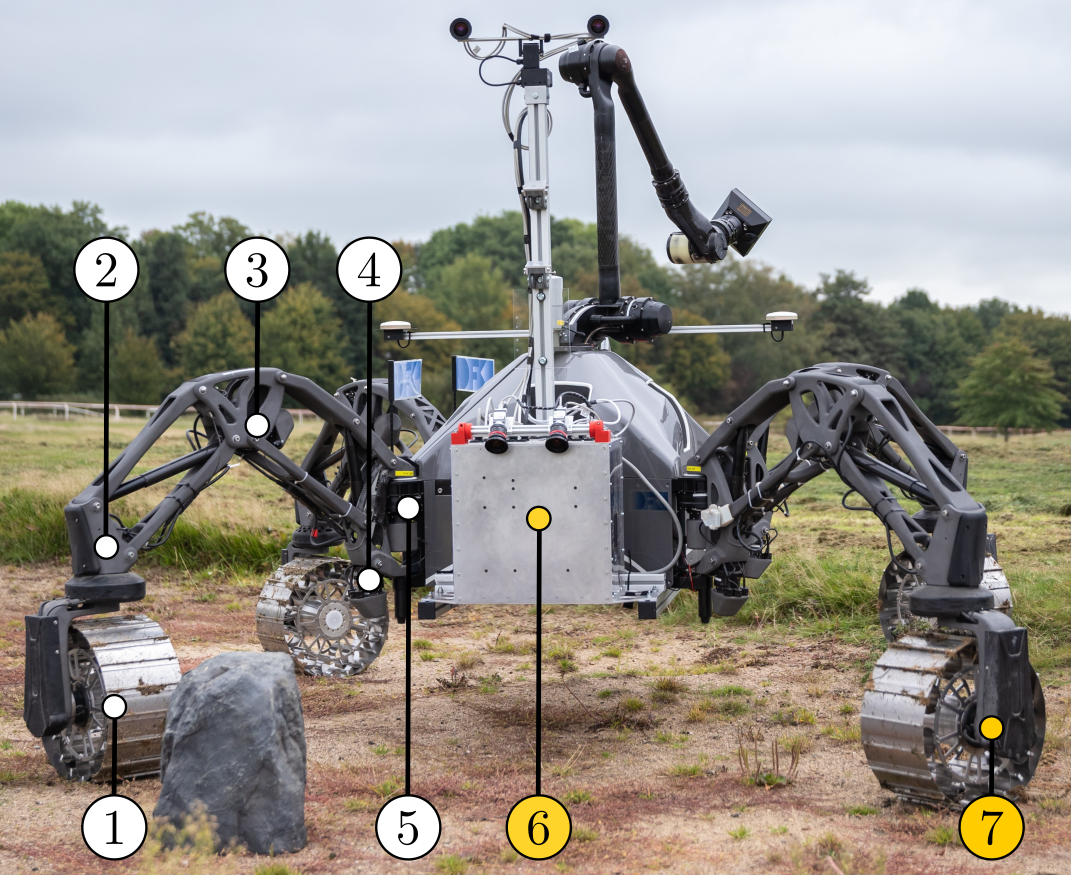
\includegraphics[width=0.9\columnwidth]{../figures/terrain_classifier_sensor_inputs.png}
       }
   \qquad \qquad
   \subcaptionbox{
       \label{fig:MCS}Motion Control System of SherpaTT
       }
       {
           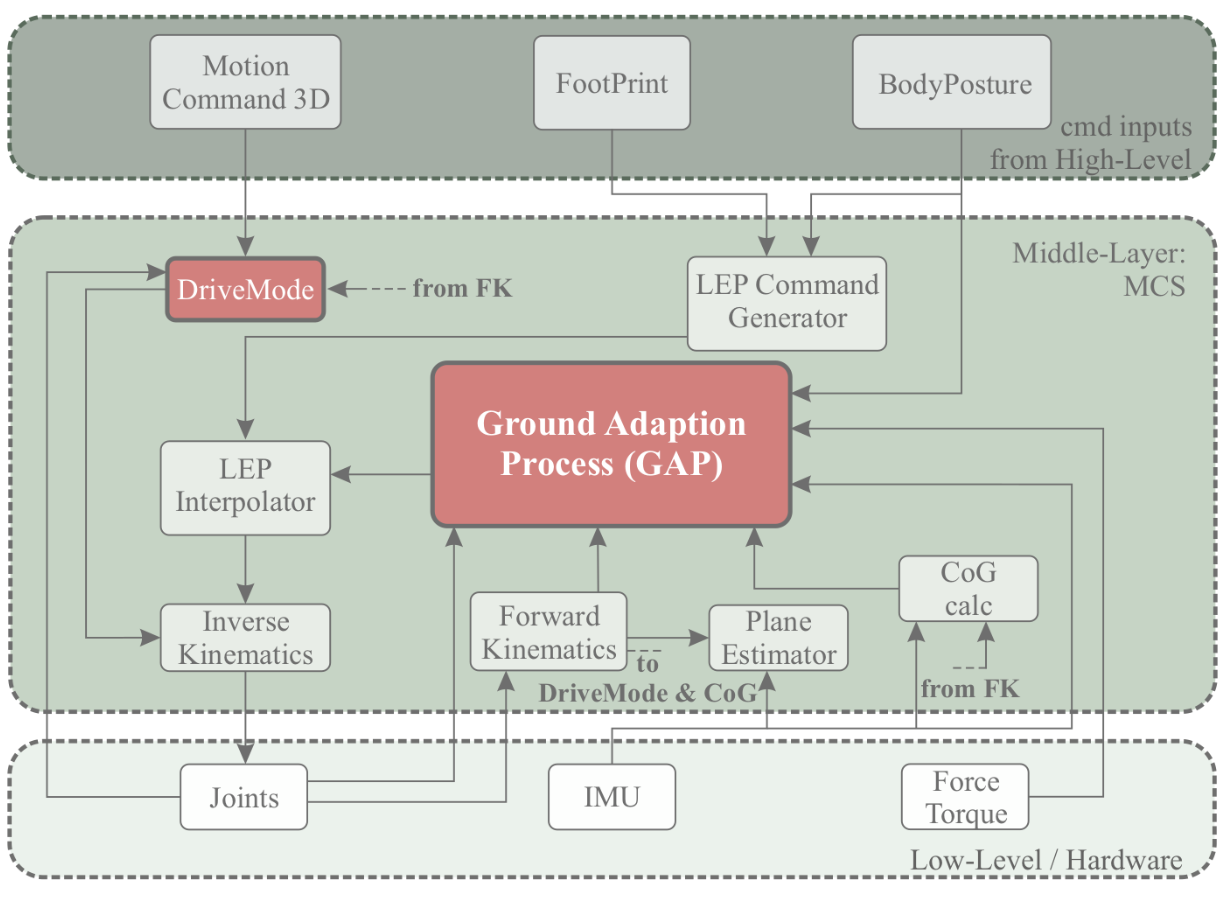
\includegraphics[width=\columnwidth]{../figures/MCS-Structure.png}
       }
   \caption{\label{fig:Loco}(a) Input features for the terrain classifier originate from the following actuators (1)-(5) and sensors (6)-(7) on SherpaTT: (1) wheel drive, (2) wheel steering, (3) linear knee, (4) linear hip, (5) pan hip, (6) IMU, (7) Force-Torque. (b) Simplified layout of the Motion Control System of SherpaTT \citep{cordes_phd_2018}.}
\end{figure*}

SherpaTT is a hybrid wheeled-leg rover with an actively articulated suspension system. Its locomotion control system provides the basis for advanced locomotive capabilities with the ability to adapt to different terrain types \citep{cordes2018}. The rover is designed to operate in unstructured environment. It features terrain adaption based on force torque sensors inputs, trajectory control and path planning as well as environment reconstruction through data fusion of extereoceptive and proprioceptive data. The placement of the sensors that provide proprioceptive input data to the terrain classifier on SherpaTT is shown in Figure~\ref{fig:SensorInputs}. The purpose of the high mobility platform is to access scientifically interesting areas on planetary bodies in a safe and autonomous way. Besides the enhanced locomotion system, SherpaTT benefits of its advanced motion control system (MCS). The MCS guarantees controlled articulation of the complex kinematic suspension system at any time. It is implemented as a middle-layer between high-level processes and the low-level hardware layer, as shown in Figure ~\ref{fig:MCS}. The layered architecture of SherpaTT can be described as \citep{cordes2018}:

\begin{itemize}
    \item \textbf{High-Level:} the autonomy level of the robot’s control system. Resembles i.a. navigation, mapping and path planning software. Related behaviors are independent of the physical states of the robot.
    \item \textbf{Middle-Layer:} resembles an abstraction of the physical robot. Handles command inputs from the operator or high-level processes and calculates according joint movements. It reacts to sensor inputs and thereby assures system stability for example by monitoring the position of the Center of Gravity (CoG) to avoid tip-over.
    \item \textbf{Low-Level:} close to the physical hardware. This comprises sensors and local joint controllers, for example PID controllers for position or velocity control of individual joints. Besides providing commands to the wheel drive actuators, the MCS design aims to mimic a passive suspension with controllable properties.
\end{itemize}

\subsection{Development Tools}

The control and perception software on SherpaTT exchanges data and information through the Robotics Construction Toolkit (Rock) framework. 
The framework not only provides wrapping mechanisms for the libraries and its communications, but also offers the possibility to enforce realtime execution of the control loops, when using a realtime supporting Linux kernel. 
Rock incorporates a set of useful tools for development, testing and evaluation of software libraries (e.g. runtime data exchange statistics and visualization). 
In particular, tools for data logging, replaying and memory-signature based data selection from data streams have been employed in this implementation. 

% Challenges
Data selection at runtime is one of the key features addressed by the middleware. 
The problem consists in generating matrices of synchronous sample values for classification online from data streams with multiple frequencies.
Each data stream relevant for the classification contains in addition to the relevant data, data which has to be filtered out (e.g. timestamps) since it is useless for the classification.
The library \emph{type to vector}\footnote{Type to vector: \url{https://github.com/rock-data-processing/data_processing-orogen-type_to_vector}} is used to select the relevant fields of data types in the samples of the data stream. 
It uses memory type descriptions of the samples which contain relevant data to select from the incoming streams only the relevant attributes and stack them into the input matrix. 

The synchronicity of the input data to the classifier is achieved by labeling sensor data with timestamps at acquisition time.
Data streams can have different update rates, but the input matrices need data from multiple sources at the same rate, therefore a strategy is needed to discard or interpolate data. 

The Rock logging mechanism is used to store the sensor and fused data streams on a hard drive for later offline use (i.e. data collection) while traversing. 
Two further tools are employed to process the logged data offline: \emph{rock-replay} for testing the runtime functionality on the development environment and \emph{pocolog to msgpack}\footnote{Pocolog to Msgpack: \url{https://github.com/rock-core/tools-pocolog2msgpack}} to select and prepare the data, so that it can be employed for training and testing the classifier.
\emph{pocolog to msgpack} converts data from its Rock binary representation to the almost universal \emph{msgpack} format.
Moreover, \emph{pocolog to msgpack} allows for the conversion of logged data into Python data frames, the widely used data science and machine learning format. 
Finally, the runtime inspection tools of Rock are utilized to monitor the processing time of the classifier, the connections between separate software components and to visualize the coherence of all input data streams. 

\subsection{Terrain Classifier}
% Background and approach

In order to classify three terrain types using proprioceptive sensor data, the supervised machine learning algorithm Support Vector Machine (SVM) is utilized \citep{cortes1995}. 
The application requires the training of a SVM classification model that is later used to classify n-dimensional data points.
The model's dimensions are called \emph{features} and they correspond to the inputs that are used to estimate the class. 
During training the SVM adapts the boundaries among the different classes. The greater the separation between the classes, the clearer the classification of data points will be.
In order to achieve a maximum separation between data classes, the optimal features, computed from the sensor data, need to be identified. 
In other words, a feature selection process allows to identify the most critical set of input data to the classifier. 
%features differs in performance  
%feature selection

\paragraph*{Model Training}
%\subsubsection{Model Training}
Generally, a SVM aims to separate data into multiple classes. 
In geometrical terms it divides the data with a n-dimensional hyperplane, the \emph{decision boundary}. 
The hyperplane parameters, or \emph{weights}, are iteratively optimized to allow for the largest distance between the hyperplane and the nearest data points which eventually are the support vectors.  
By changing the dot-product calculation, referred to as the kernel trick, within the underlying geometrical condition various correlations of the data's dimensions can be recognized. 
Correlation can be obtained through a polynomial or a Gaussian radial based function. However, the most simple option is linear correlation.
The generated set of weights is referred to as \emph{classification model} and the generation process as such is called \emph{training}.%\cite{kuhr2021}
%OvA multiclass strategy



%\subsubsection{Model Testing}


\paragraph*{Model Testing}
Before deploying the model, its classification performance can be measured using labeled data.
This testing process obtains performance measures that are typically visualized with \emph{confusion matrices}. 
A description of the three class confusion matrix used to present the results in this work is depicted in Figure~\ref{fig:CMdescrpit}, where $T$ stands for True (correct) and $F$ for False (wrong).
The three evaluated aspects or performance measures are \emph{precision}, \emph{recall} and \emph{accuracy}.
The step of processing a sample and providing a classification label is also referred to as \emph{prediction}.

\vspace{50px}

\begin{itemize}
\item \textbf{Accuracy} measures the overall percentage of correctly classified samples: 

    \begin{equation}
        \frac{T\textsubscript{overall}}{(T+F)\textsubscript{overall}} 
    \end{equation}

\item \textbf{Recall} measures for each set of samples of each class the correctly classified percentage:
%: Out of all samples that belong to an actual class does the classifier classify the correct class 

    \begin{equation}
        \frac{T\textsubscript{class}}{(T+F)\textsubscript{actual class}}
    \end{equation}

\item \textbf{Precision} measures for each set of predictions per class the percentage of correct predictions: 
%: Out of all classifications that the classifier assigns to one class does the classifier classify correctly

    \begin{equation}
        \frac{T\textsubscript{class}}{(T+F)\textsubscript{predicted class}}
    \end{equation}
    
\end{itemize}


\begin{figure*}[!htbp]
    \centering
    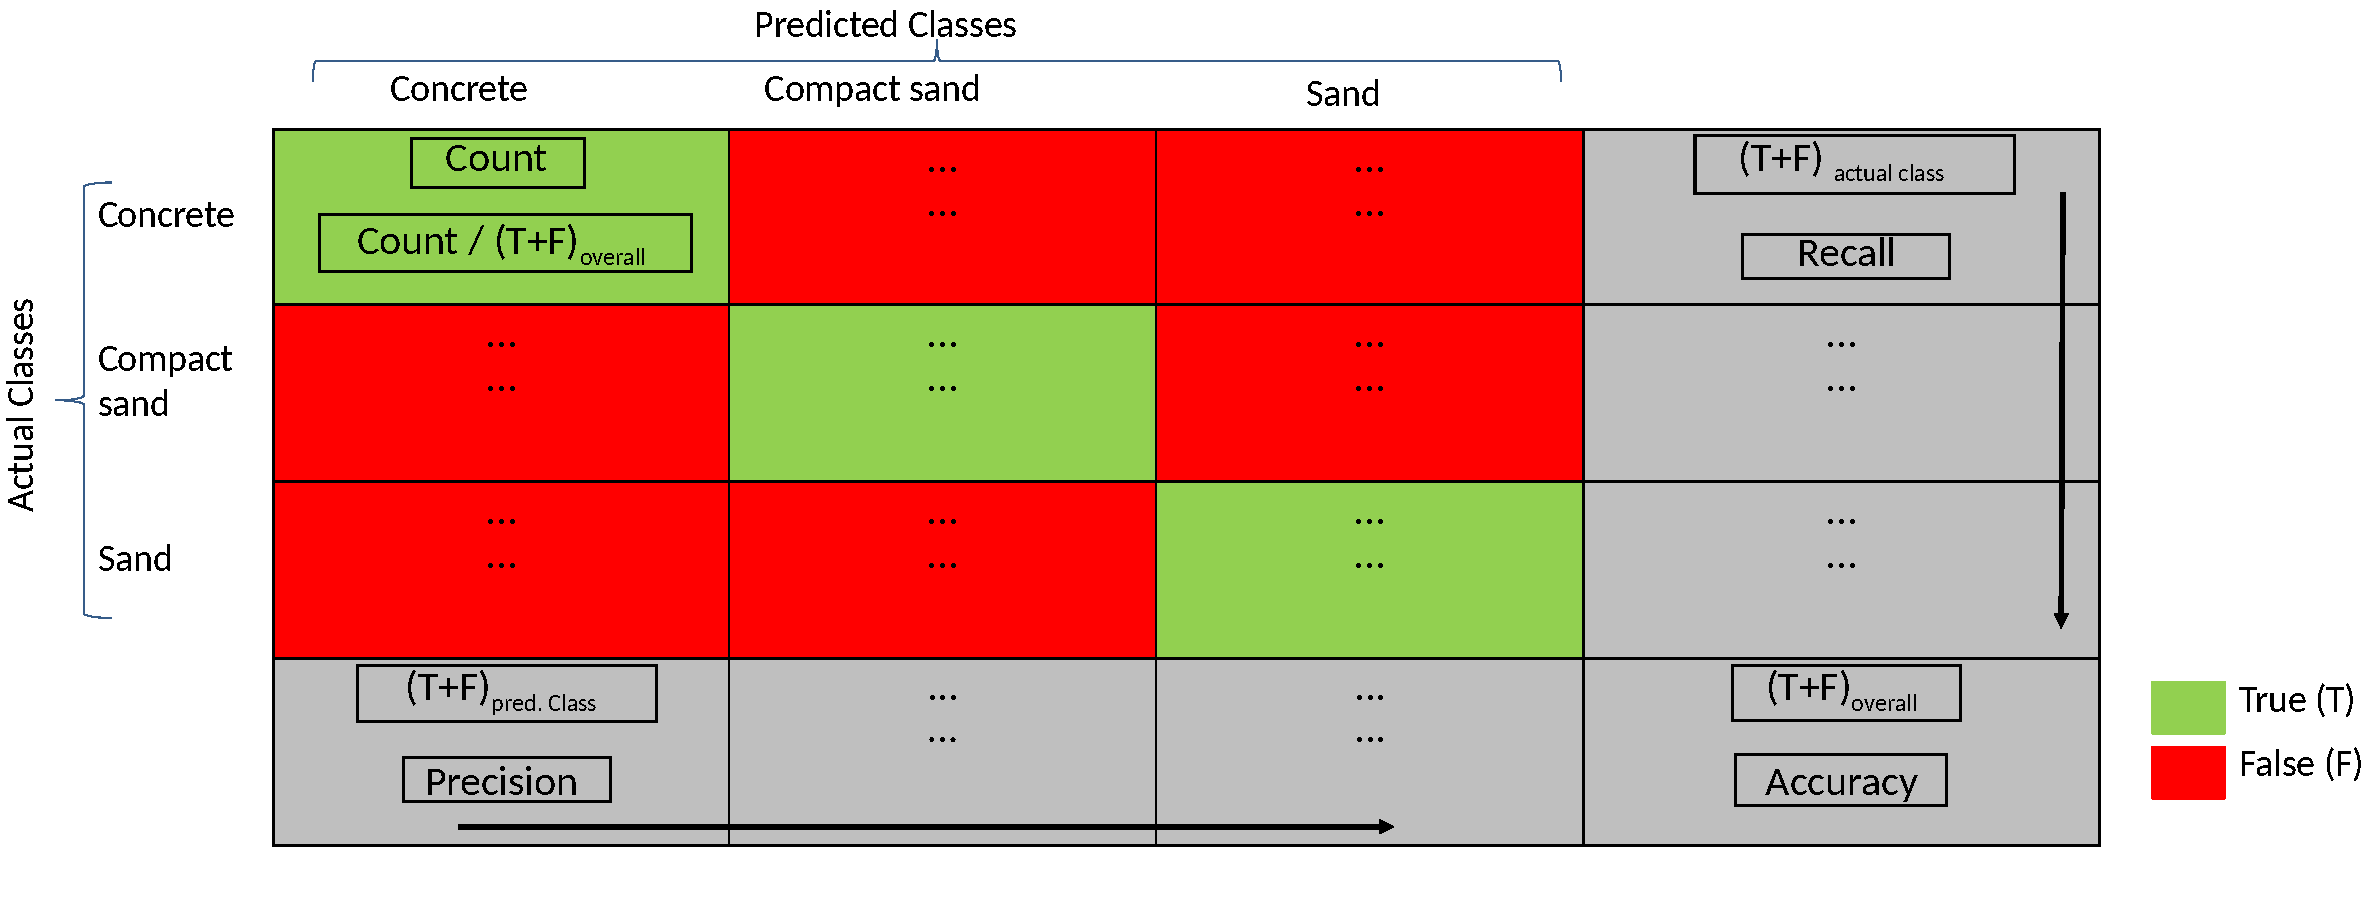
\includegraphics[width=\textwidth]{../figures/CM_Description.pdf}
    \caption{\label{fig:CMdescrpit} Confusion matrix used to visualize the performance measures, \emph{Precision}, \emph{Recall} and \emph{Accuracy}, of the classifier \citep{kuhr2021}.}
\end{figure*}


%\subsubsection{Feature Selection}
\paragraph*{Feature Selection}
For computational reasons and simplicity, it is desired to reduce the dimensionality by selecting the most critical features for the  classification task.
A large set of statistical moments of the features is considered within the selection process. 
The features can represent direct sensor parameter as well as physical parameters like mechanical and electrical power, friction coefficients and the wheel speed deviation of each wheel in relation to the others. 
The proprioceptive sensor data used to calculate the features is listed in Table~\ref{table:features1} which is based on \citep{Dimastrogiovanni2020}.
The input data is received from the Motion Control System (MCS), Joint Deployment (JD) and Sensors Deployment (SD). 
All forces and torques are represented within the Body Coordinate System (BCS).

\pagebreak

\begin{center}
\bottomcaption{Proprioceptive inputs and supplying datastream.}
\label{table:features1}
\tablefirsthead{
   \textbf{Datastream}        & \textbf{Feature}       & \textbf{Symbol} \\ \hline
   }
\begin{supertabular}{ccc}
        \quad  & \quad               & \quad \\[-5pt]
        MCS & Longitudinal Force     &  $F\textsubscript{x}$  \\
        MCS & Vertical Force         & $F\textsubscript{z}$   \\ 
        MCS & Drive Torque y-axis    & $T\textsubscript{y}$   \\ 
        JD  & Motor Current          & $I$                    \\ 
        JD  & Voltage                & $V$                    \\ 
        JD  & Dutycycle              & $d\textsubscript{pwm}$ \\ 
        JD  & Angular Wheel Velocity & $w$                    \\
        SD  & Acceleration X         & $a\textsubscript{x}$   \\ 
        SD  & Acceleration Z         & $a\textsubscript{z}$   \\ 
\end{supertabular}
\end{center}

\begin{center}
\bottomcaption{Optimal feature set for the classification of terrain types by SherpaTT. The set includes the statistical calculation of mean (M) and standard deviation (SD) per terrain patch.}
\label{table:features2}
\tablefirsthead{
   \textbf{Statistical}        & \textbf{Feature}       & \textbf{Symbol} \\ \hline
   }
\begin{supertabular}{ccc}
     \quad  & \quad                        & \quad \\[-5pt]
     M,SD	&  Longitudinal Force	       & F\textsubscript{x} \\ 
     M,SD	&  Drive Torque	around y-axis  & T\textsubscript{y} \\ 
     M,SD	&  Drive Current	           & I \\  
     M,SD	&  Acceleration X	           &  a\textsubscript{x}\\ 
     M,SD	&  Acceleration Z	           & a\textsubscript{z} \\ 
     M,SD	&  Mechanical Power	           & P\textsubscript{m} \\ 
     M,SD	&  Electrical Power	           & P\textsubscript{e} \\ 
     M,SD	&  Friction Coefficient 1	   & \textmu \textsubscript{1} \\ 
     M,SD	&  Friction Coefficient 2      & \textmu \textsubscript{2}\\ 
     M,SD	&  Friction Coefficient 3	   & \textmu \textsubscript{3}\\ 
     M	    &  Angular Wheel Velocity	   &  w      \\ 
     SD    	&  Speed Deviation	           & $\Delta$w\\ 
\end{supertabular}	
\end{center}

Using the inputs in Table~\ref{table:features1}, the physical features listed in Table~\ref{table:features2} are statistically determined for each patch of terrain to be classified.
The statistical moments, mean, variance, skewness and kurtosis are initially evaluated. 
A selection of the most useful features for the classification is done using the WB index and the Pearson coefficient to reduce the dimensionality of the data. The equations for physical features calculation and for most critical features selection are both detailed in \citep{Dimastrogiovanni2020}.

%\subsubsection{Linear Discriminant Analysis}
%copy paste from thesis
%\paragraph*{Linear Discriminant Analysis}
%Besides speeding up the training and reducing the required amount of data during runtime, the reduction of feature dimensionality can help for data visualization. 
%Linear Discriminant Analysis (LDA) reduces the number of dimensions down to the three or two more representative. 
%This makes it possible to plot a high-dimensional data set on a graph and through this visually gain information about patterns. 
%
%To achieve this, LDA identifies the axis that accounts for the largest amount of variance of different class's data. 
%It thereby represents a similar method as the Principle Component Analysis (PCA) with the difference that LDA recognizes the class labels when identifying the variance. 
%As a next step, LDA identifies the axis that lays orthogonal to the first one. 
%Therefore, the second axis accounts for the largest amount of remaining variance. 
%The maximum number of orthogonals, linear discriminants, depends on the number of dimensions within the data set.\cite{kuhr2021}
%
